\documentclass[a4paper,12pt]{article}

\usepackage[english,brazil]{babel}
\usepackage[utf8]{inputenc}
\usepackage{icomma}
\usepackage{amsmath}
\usepackage{makecell}
\usepackage{graphicx}
\usepackage{fancyhdr}
\usepackage{url}
\renewcommand{\baselinestretch}{1.5}
\usepackage{titling}
\usepackage{geometry}
\usepackage{subfigure}
\geometry{
 a4paper,
 left=35mm,
 right=15mm,
 top=1in,
 bottom=1in,
}
\usepackage{amsmath}
\usepackage{amssymb}
\usepackage{subfigure}
\usepackage{multirow}
\usepackage[table]{xcolor}
\usepackage[backend=bibtex,style=ieee,sorting=none]{biblatex}
\usepackage{algorithm}
\usepackage[noend]{algpseudocode}
\usepackage{pdfpages}
\usepackage{enumerate}
\bibliography{main}
\newcolumntype{C}{>{\centering\arraybackslash}p{1em}}


\newpage

\begin{document}
\selectlanguage{brazil}

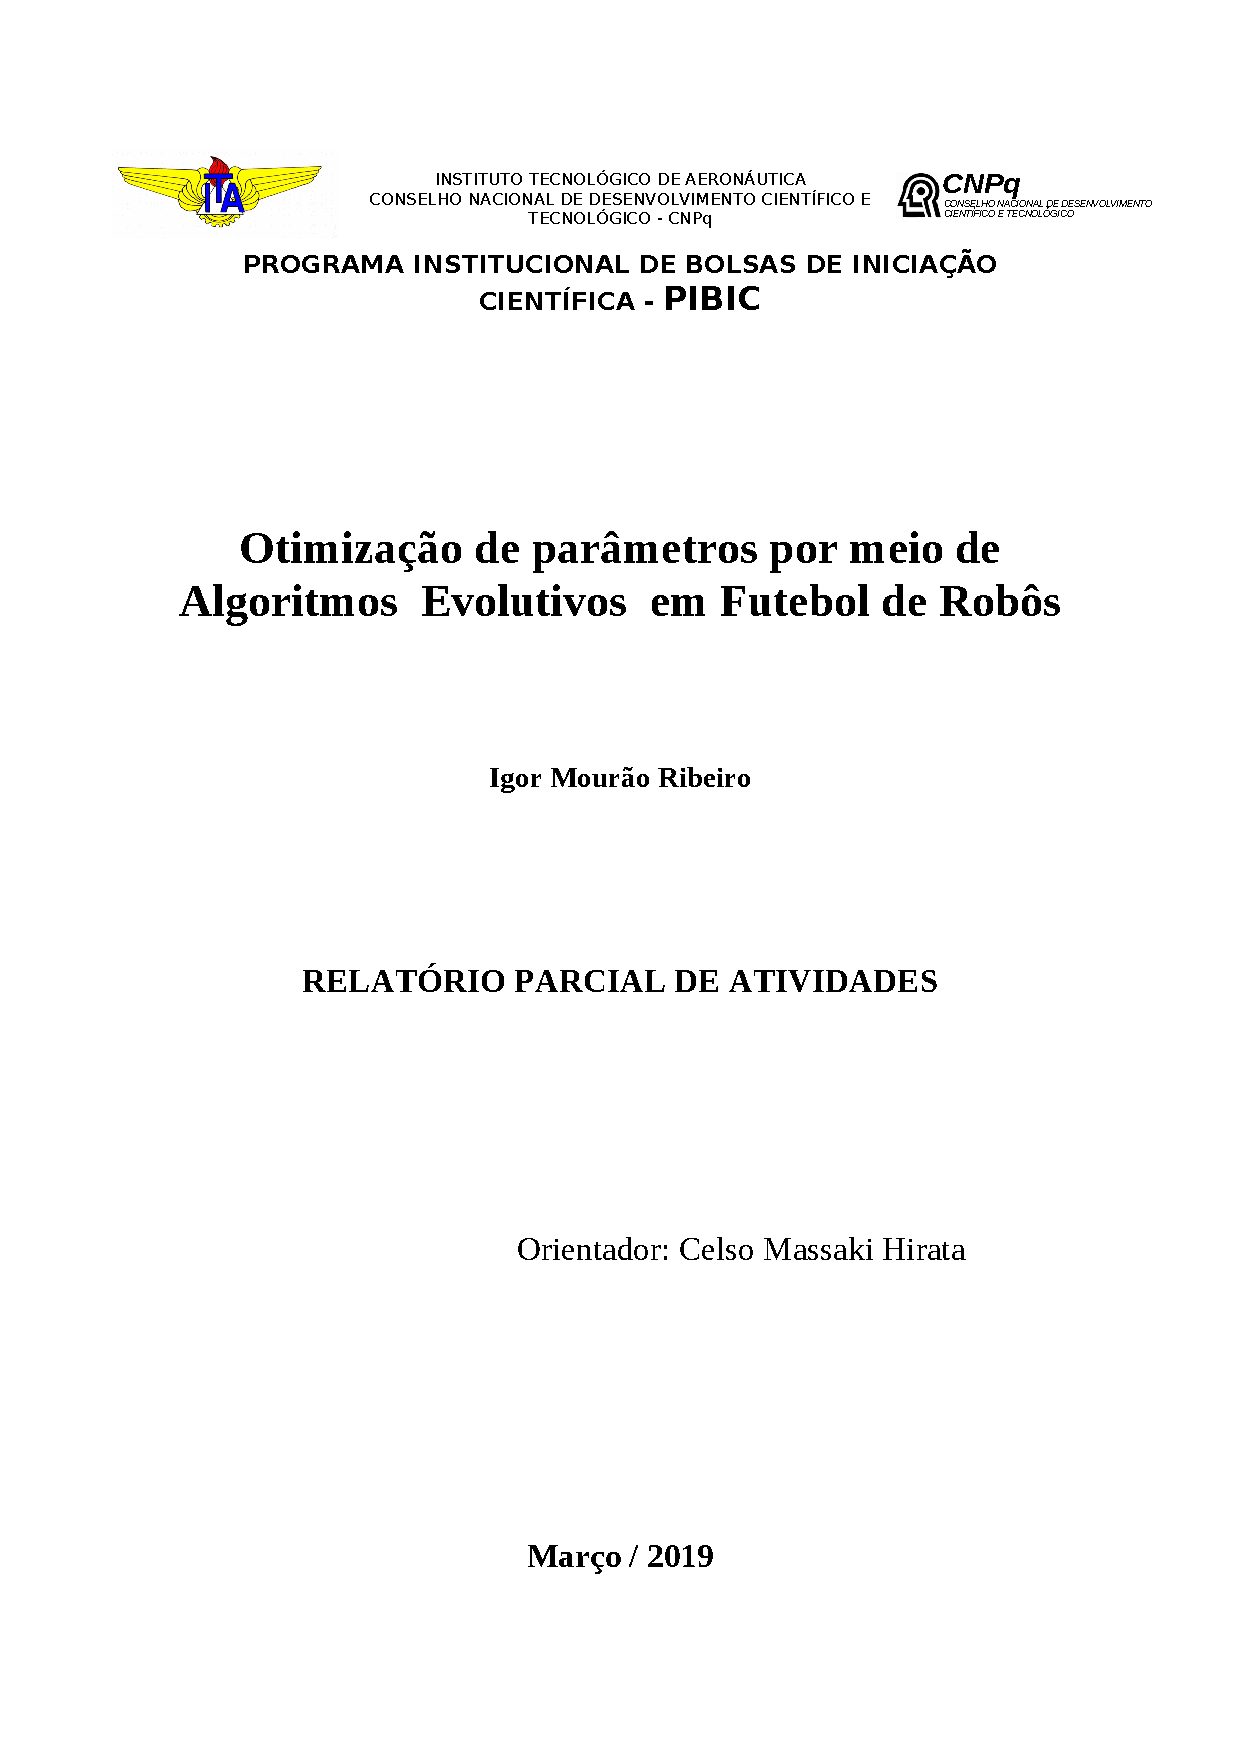
\includepdf[pages={1-},scale=1]{Inicio.pdf}


\tableofcontents

\newpage

\section{Resumo do Plano Inicial}
\label{secao:plano_inicial}

O objetivo deste trabalho é desenvolver e implementar um algoritmo para a otimização de parâmetros de um time composto por três robôs diferenciais. O contexto é uma partida de futebol segundo a Competição Brasileira de Robótica (CBR), categoria IEEE Very Small Size Soccer (VSSS). Por meio da criação de métricas e testes automatizados para medir o desempenho do time de robôs em diversas situações de jogo, pode-se utilizar algoritmos evolutivos para fazer a otimização de parâmetros relevantes, como os relativos ao planejamento de trajetória. Visa-se utilizar os algoritmos aqui implementados pela equipe da ITAndroids, que representa o ITA, em competições nacionais e internacionais, como na competição Latin America Robotics Competition (LARC)/CBR.

Planejamento:
\begin{itemize}

\item 1o Bimestre (ago / set): Estudo da literatura e revisão bibliográfica sobre o tema de otimização de parâmetros para robôs jogadores de futebol.

\item 2o Bimestre (out / nov): Seleção de métricas a serem utilizadas e implementação inicial do código.

\item 3o Bimestre (dez / jan): Implementação dos testes e simulações para as métricas escolhidas. Redação do relatório parcial.

\item 4o Bimestre (fev / mar): Análise e implementação do algoritmo escolhido.

\item 5o Bimestre (abr / mai): Análise do desempenho da otimização para o planejamento de trajetórias. Ajuste do algoritmo para melhores resultados.

\item 6o Bimestre (jun / jul): Redação do relatório final. Redação do artigo para o ENCITA. Teste final para o software completo no robô real, com todas as áreas do projeto operantes.

\end{itemize}

\section{Resumo das Atividades Realizadas}
\label{secao:atividades_realizadas}

Ao longo dos dois primeiros meses, foram realizados estudos e foi decidido que será usado o algoritmo Covariance Matrix Adaptation Evolution Strategy (CMA-ES) para a otimização de parâmetros. Esse algoritmo foi escolhido dentre de opções como NEWUOA e o algoritmo de Broyden–Fletcher–Goldfarb–Shanno (BFGS). Mais detalhes sobre esses dois últimos métodos pode ser encontrada, respectivamente, em \cite{NEWUOA} e em \cite{BFGS}. Para uma descrição sobre a eficácia do algoritmo CMA-ES no contexto de futebol de robôs, pode-se encontrar na referência \cite{CMA-ES}.

Ao longo do segundo e terceiro bimestres, a base do algoritmo foi implementada utilizando Matlab \cite{matlab}, que é uma linguagem especializa em algébra linear utilizada pela equipe. Foi, em seguida, realizada a escolha e codificação das métricas a serem utilizadas para medir o desempenho de uma determinada situação de jogo.

O algoritmo foi, em seguida, implementado e integrado com o restante do código da equipe. Após algumas iterações, os parâmetros relativos ao planejamento de trajetória do robô foram otimizados e testados em simulações. Os resultados se mostraram satisfatórios e condizentes com o previsto.

Os resultados obtidos foram efetivos como mostrado na LARC, ocorrida entre os dias 6 a 10 de novembro de 2018. O algoritmo mostrou que o planejamento de trajetórias da equipe, em conjunto com o controle do robô, estavam muito precisos, fato que concedeu à equipe uma vantagem decisiva na competição. A equipe da ITAndroids conquistou o primeiro lugar da competição, sendo a sua classificação mais alta na categoria Very Small Size Soccer da história.

\section{Descrição do Problema}
\label{secao:enunciado_problema}

No contexto do futebol de robôs, a tomada de decisão traz muitos desafios. A estratégia consiste no fato de se implementar um algoritmo que consiga utilizar o planejamento de trajetórias do robô da melhor maneira possível. Isso nos traz a um desafio de nível de abstração mais alto: decidir qual a melhor decisão que cada robô pode tomar em um certo momento considerando limitações de trajetórias possíveis de serem seguidas. A figura \ref{fig:vss_ele} mostra a placa eletrônica do robô utilizado. 

\begin{figure}[H]
	\centering
	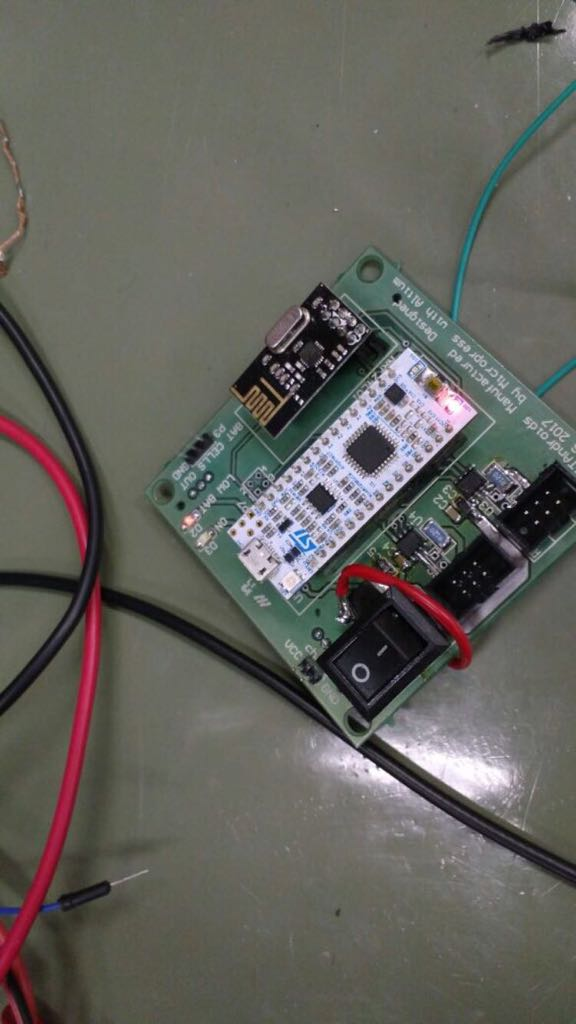
\includegraphics[width=0.5\textwidth]{figures/vss_ele.jpg}
   \caption{Placa eletrônica de um robô Very Small Size.} \label{fig:vss_ele}
\end{figure}

Nesse projeto, trabalhou-se com os robôs da competição IEEE Very Small Size (VSS): uma competição de futebol de robôs completamente automatizada em que cada robô tem como tamanho máximo um cubo de 7,5 cm de aresta. O campo de futebol possuil 1,5 m de comprimento e 1,3 m de largura. Cada time tem 3 jogadores: que podem assumir posições dinâmicas, como goleiro e atacante, ao decorrer de uma partida. Uma câmera proporciona a visão aérea com as posições de todos os elementos da partida. As regras completas podem ser lidas em \cite{cbr2008}.

\begin{figure}[H]
	\centering
	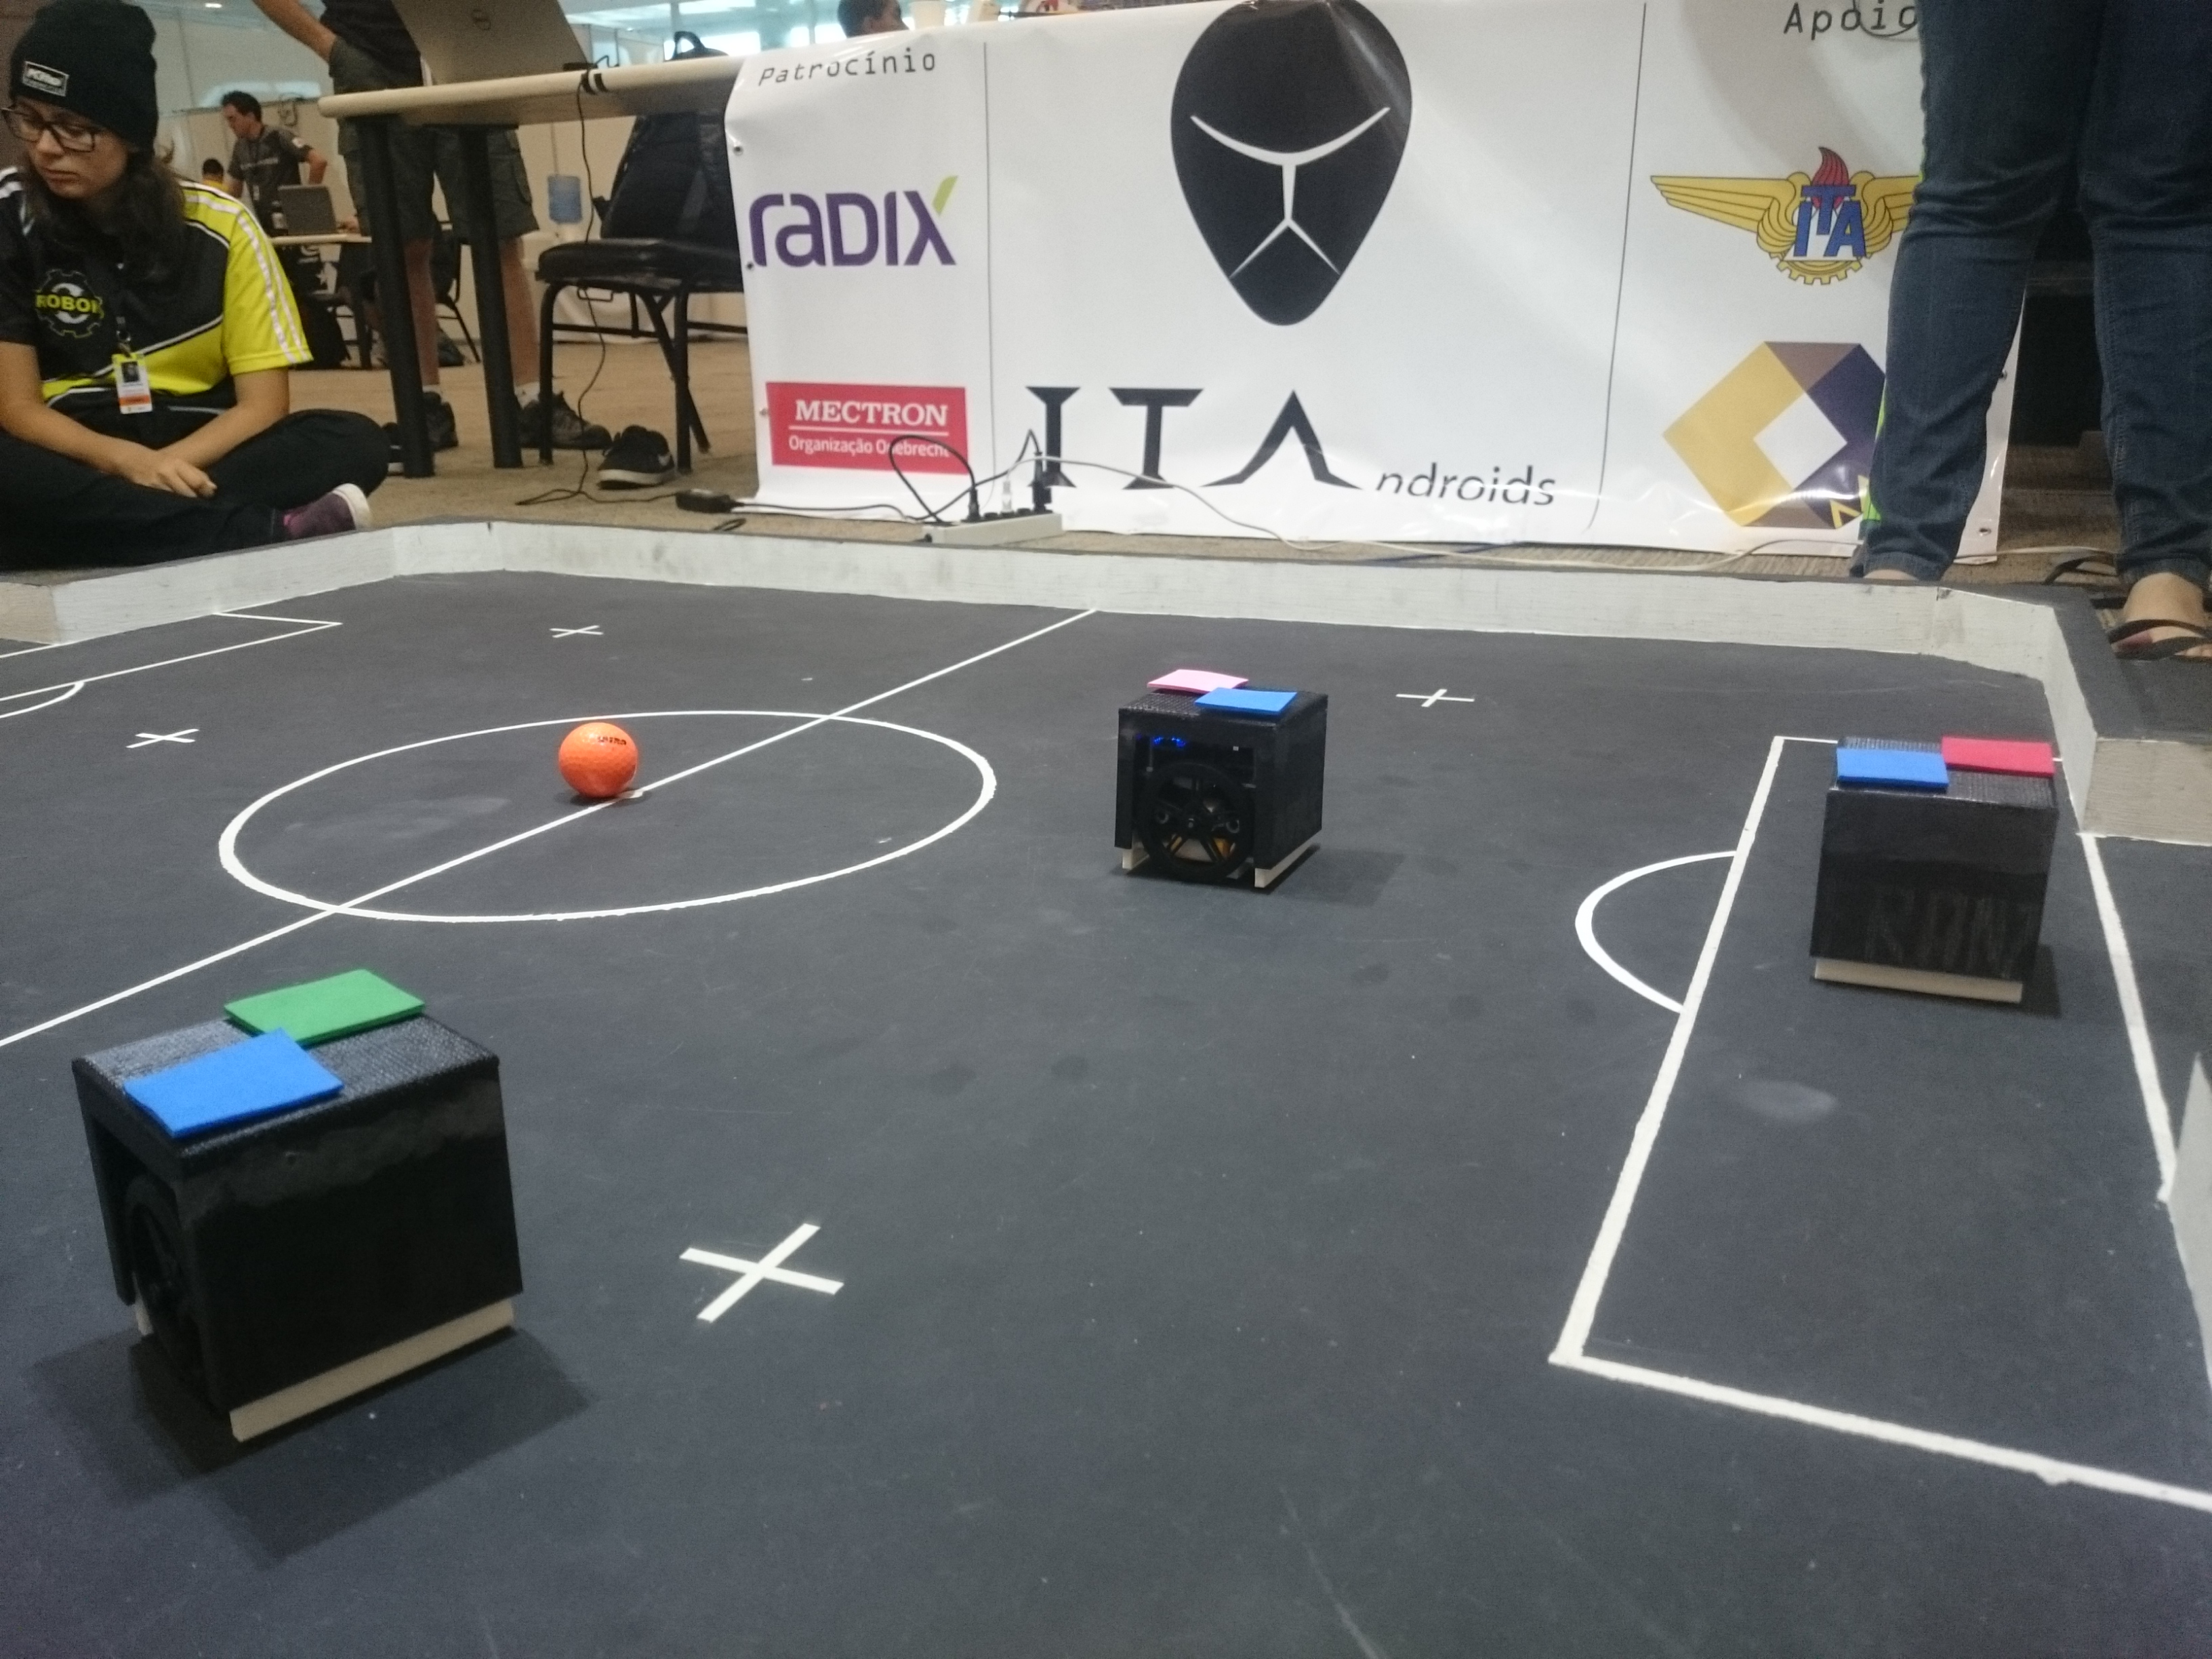
\includegraphics[width=0.5\textwidth]{figures/vss.JPG}
   \caption{Robôs da ITAndroids da categoria IEEE VSSS.} \label{fig:vss}
\end{figure}

A figura \ref{fig:vss} mostra os robôs usados nas competições. A visão computacional utilizada pela equipe ITAndroids pode ser encontrada com mais detalhes em \cite{tasinaffo_ic} e utiliza uma câmera no topo do campo que repassa informaçãoes para um computador processar, como visto na figura \ref{fig:funcioamento}.

\begin{figure}[H]
	\centering
		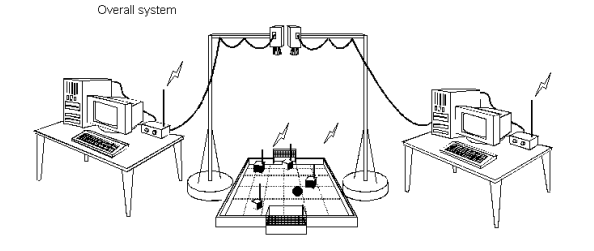
\includegraphics[width=0.7\textwidth]{figures/overview.png}
  \caption{Representação do funcionamento técnico de um jogo de VSS.}
	\label{fig:funcioamento}
\end{figure}

Cada robô foi projetado com duas rodas laterais e duas esferas livres à frente e atrás para manter o equilíbrio. Essa característica o torna um robô diferencial. Ou seja, temos o controle sobre as velocidades linear e angular, mas não é possível mover o robô para os lados. A linguagem utilizada para o projeto foi C++, pois é uma linguagem que tem uma velocidade de execução alta e tem escalabilidade descente para um projeto grande. 

Nesse contexto, surgem várias questões a serem resolvidas para se ter um time vencedor. Nesse projeto, será abordado o seguinte problema de estratégia: dada a posição e a velocidade de cada robô no campo, da bola e da direção que os nossos robores estão (não é possível descobrir a posição dos robôs oponentes, pois não sabemos a distribuição de cores que eles usam no seu topo), deve-se escolher qual posição o robô irá, com qual controlador  e qual planejamento de trajetórias utilizar. Deve-se também montar um plano para ações futuras, planejando uma sequência de posições que o robô deve ir para efetuar um gol.

O algoritmo de estratégia deve executar em tempo de execução de, no máximo, 16 ms para todo o time, que é o tempo de amostragem da câmera. A maior parte desse tempo é gasto com o planejamento de trajetórias usado, que é o Rapidly-exploring Random Tree (RRT). O tempo para cada execução de um RRT é de 1 ms, de acordo com \cite{franzoni_rrt}, limitando a em torno de um limite de doze chamadas do algoritmo por execução completa da estratégia, com uma margem de erro trinta e três porcento. Ressalta-se a importância de não ultrapassar esse tempo máximo, já que se isso acontecer perde-se uma imagem da câmera e o funcionamento do jogo é realizado de forma atrasado.

Deve-se, então, ser montado um esquema de posicionamento dinâmico em que não existam nem atacante, nem zagueiro, nem goleiro fixos, mas sim, que as posições dependam e se adaptem com a posição de jogo, garantindo que os três jogadores possam estar mais bem posicionados e tenham liberdade para escolherem suas próximas ações.

Para resolver esse problema, foi escolhido como principal algoritmo para a tomada de decisão a Behavior Tree, embasado na decisão de um time referência no futebol de robô mundial na categoria Small Size League \cite{ssl}, o Near East University team: the NEUIslanders \cite{NEUIslanders_ssl}.


\subsection{Behavior tree}

Para se construir uma BT, é preciso primeiro entender o básico de sua estrutura. Uma BT é uma Árvore no sentido dado pela teoria dos grafos, como explicado em \cite{west2001introduction}. Por definição, cada nó dessa árvore será chamado de behavior.

Os nós de uma Behavior Tree são diferenciados em dois tipos: os nós folhas, que são os nós da árvore que não tem filhos e os nós compostos, que podem ter um ou mais filhos.

Todos os nós retornam, no final de sua execução, um dos três estados a seguir: TRUE, FALSE ou RUNNING, para indicar, respectivamente, que o nó foi terminado com sucesso, que foi terminado sem sucesso ou que o algoritmo deve executar esse nó por pelo menos mais uma iteração.

\subsubsection{Nó Folha}

Os nós folha são os nós terminais da Árvore e eles que representam as ações mais baixo níveis e concretas da estratégia. São divididas em dois tipos: nós de ação e nós condicionais.

\textbf{Nó de Ação} São os nós que de fato realizam uma ação, como se movimentar até a bola.

\textbf{Nó condicional} São nós que apenas retornam um estado sem realizar nenhuma ação concreta, como checar se o time está atacando. São usados para controlar quais nós serão executados em conjunto com os nós compostos.

\subsubsection{Nó composto}

Nós compostos são os nós intermediários da árvore, que  são resposáveis por escolher quais os nós que serão executados. São completamente reutilizáveis no sentido que apenas uma implementação de cada tipo de nó composto deve existir e ela poderá ser usada em diversas partes do código. Os principais tipos desses nós que foram usados para a estratégia estão listados a seguir:

\textbf{Selector Behavior} Nesse behavior, é selecionado um de seus filhos para ser acessado a seguir. Ele é usado quando tem-se várias maneiras de se realizar uma mesma ação e deve-se escolher a melhor delas em uma determinada situação. Ele funciona executando os filhos em uma determinada ordem e, assim que um dos filhos retorna TRUE ou RUNNING, esse nó retorna o mesmo valor. Se um filho retornar FALSE, o próximo filho será executado. Caso nenhum filho seja sucedido ou retorne que deve ser executado mais um vez, o nó retorna FALSE.

\textbf{Sequence Behavior} Esse nó executa cada um dos seus filhos em uma sequência bem definida e fixa. Ele é usado para fazer ações sequenciadas para completar um objetivo maior, por exemplo: chutar a bola para o gol oponente requer que o robô aliado esteja atrás da bola, o que significa que chegar atrás da bola e, em seguida, chutar a bola representam ações sequenciadas. Ele funciona de forma que, quando um filho retorna RUNNING ou FALSE, o behavior retorna o mesmo valor e, quando um filho retorna TRUE, ele avança para o próximo filho. Se todos os filhos retornarem TRUE, o behavior é bem sucedido e também retorna TRUE.

\textbf{Parallel Behavior} O objetivo desse nó é executar todos os seus filhos ao mesmo tempo, fato que pode ser obtido ao utilizar-se de processamento paralelo ou não. Na implementação desse trabalho foi usado a versão não paralela do algoritmo. Se um filho retorna FALSE, o behavior retorna FALSE. Se todos os filhos retornarem TRUE, o behavior retorna TRUE. Em todas as outras situações, o behavior retorna RUNNING e continua sua execução por pelo menos outra iteração.

\textbf{Decorator} O nome para esse behavior é inspirado no conceito de Decorator em Software Design Pattern, que pode ser explicado em \cite{hunt2013gang}. No contexto da Behavior Tree, esse nó tem apenas um filho e ele modifica o comportamento do filho de alguma maneira. Um decorador pode ser diversos tipos, mas os mais usados no projeto foram:

\begin{enumerate}
\item AlwaysFail e AlwaysSucceed: que fazem que o fiho sempre retorne FALSE ou sempre retorna TRUE respectivamente.
\item UntilFail e UntilSucceed: fazem que o fiho sempre retorne RUNNING a não ser que ele retorna FALSE ou TRUE, respectivamente.
\item Invert: muda o retorno do filho de FALSE para TRUE e TRUE para FALSE.
\end{enumerate}

\subsection{Técnico}

Uma Behavior Tree, que embora consegue modelar comportamentos complexos com facilidade, nem sempre é a melhor escolha para determinadas situações. Por isso, a estratégia foi dividida em níveis de abstrações diferentes, em que a um Técnico, representado pela classe Coach, seria responsável por escolher e administrar quais árvore cada um dos três jogadores deveria usar no momento.
Com essa implementação, tem-se um agente externo controlando a função dos jogadores por meio da escolha de uma BT, que pode ser uma árvore para um goleiro, para um principal e para um auxiliar. Isso significa que, em um dterminado momento, o técnico pode escolher que o time tenha 1 goleiro, 1 principal e 1 auxiliar a até mesmo 3 principais ao mesmo tempo. Os requisitos esperados para cada um desses papéis será abortado a seguir. Além disso, também é função do técnico escolher o papel de cada jogador a cada iteração do código, de modo que as posições dos jogadores não sejam fixas ao decorrer do jogo.

\subsection{Papéis}

Dentre os papéis que o técnico pode escolher, os escolhidos foram Goleiro, Principal e Auxiliar, conforme  proposto por \cite{egly2005decision} como papéis de alta performance.

\subsubsection{Goleiro} 

O goleiro é o jogador que deve ficar próximo ao gol aliado com o objetivo de proteger o gol de ataques oponentes. 
\begin{enumerate}
\item Ele deve ser capaz de defender bolas com velocidade lenta em direção ao gol, ao acompanham o movimento da bola seguindo a linha do gol. 
\item Essa posição deve conseguir proteger o gol de bolas rápidas, usando para isso um modelo de predição que supõe que a bola continuará em linha reta. Essa predição é necessária, pois, a altas velocidades, a taxa de amostragem da câmera não é alta o suficiente para conseguir comandar o robô apenas para seguir o movimento da bola, sendo necessário antecipar onde ela irá. A figura \ref{fig:goal_predict} mostra como essa predição linear funciona, indicando a direção da bola e o movimento que o goleiro deverá fazer para proteger o gol.

\begin{figure}[H]
	\centering
	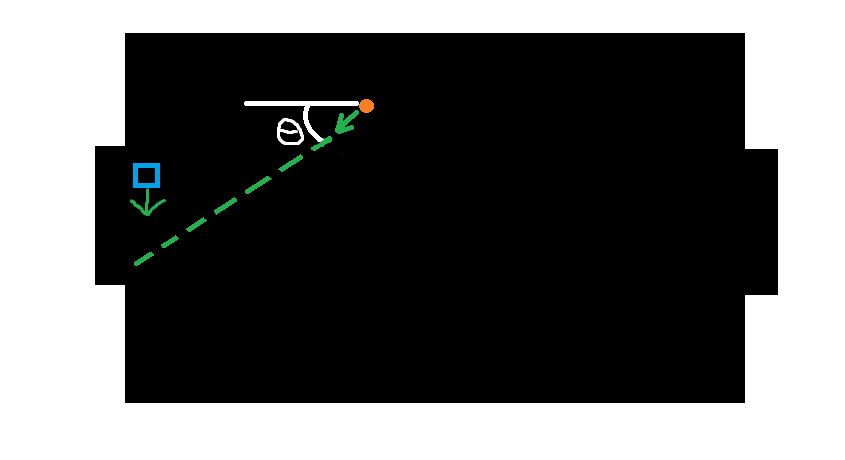
\includegraphics[width=0.8\textwidth]{figures/GoalierPredict.png}
   	\caption{Predição usada pelo goleiro para bolas rápidas.} \label{fig:goal_predict}
\end{figure}


\item Deve jogar a bola para longe do gol, por meio de rotações em torno do próprio eixo quando chegar próximo da bola para diminuir o risco de gol.
\item Deve sair do gol quando a situação não é de risco e ele chegará na bola antes de qualquer oponente. Nesse caso, outro jogador deverá se tornar um goleiro.
\end{enumerate}

\subsubsection{Principal} 

O jogador com o papel de Principal é o jogador mais ativo do time, que deve star constatemente avançando em direção a bola. Essa e o goleiro são as únicas posições que efetivamente deverao tocar na bola. Esse papel deve atender os seguintes requisitos:

\begin{enumerate}
\item deve atacar em direção ao gol oponente sempre que a bola não esteja muito próxima da parede. Isso será feito usando o planejamento de trajetórias RRT para se posicionar atrás da bola, seguido de uma rápida aceleração com a bola em linha reta em direção ao gol, de forma que o jogador leve a bola com a maior velocidade possível ao gol.
\item deve atacar pelas laterais do campo quando a bola estiver nos lados do campo de forma que ele jogue a bola para frente, sem necessariamente ter como objetivo fazer o gol, mas garantindo que o time agora esteja atacando. Para isso acontecer, será usado o RRT para se posicionar atrás da bola, seguida de uma rápida aceleração para frente.
\item deve girar em torno do próprio eixo quando estiver em um dos quatro cantos do campo. Caso esteja no ataque, esse giro fará que a bola se desloque para o meio do campo, o que pode significar que outro jogador possa pegar essa bola e levar para o gol, qualificando essa jogada com um passe entre jogadores. Caso a bola esteja em um dos cantos da defesa, o giro, além de tirar a bola da zona defensiva e a por numa posição de ataque, impedirá que a bola fique presa, fato que caracteriza em falta tiro livre segundo \cite{cbr2008}. A descrição da penalidade bola livre pode ser vista na imagem \ref{fig:bola_livre}.


\begin{figure}[H]
	\centering
	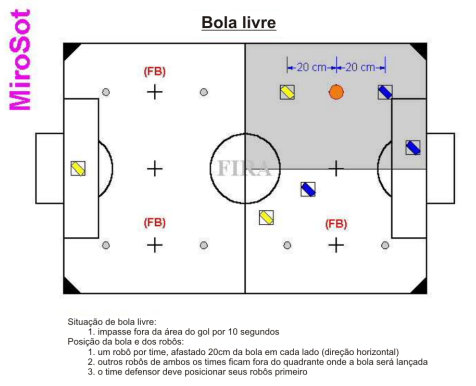
\includegraphics[width=0.8\textwidth]{figures/bola_livre.png}
   \caption{Descrição da penalidade bola livre.} \label{fig:bola_livre}
\end{figure}

 
\item deve ter comportamentos fixos e especiais para cada situações de falta, como por exemplo em um penalty, que ele deve levar a bola o mais rápido possível para um dos lados do gol para o goleiro não ter tempo de reagir e simplesmente atingir ou em um tiro livre, em que ele deve acelerar o máximo possível para chegar na bola antes do oponente. A descrição da falta do tipo penalty se encontra na figura \ref{fig:penalty}.

\begin{figure}[H]
	\centering
	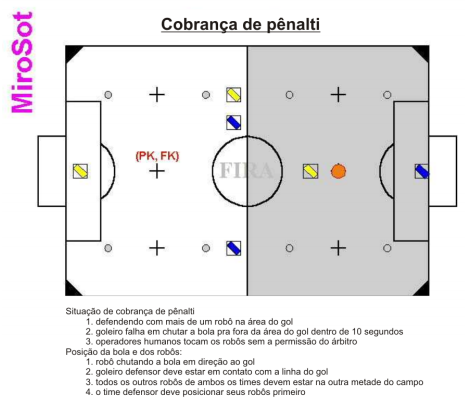
\includegraphics[width=0.8\textwidth]{figures/campo_penalty.png}
   \caption{Descrição da penalidade penalty.} \label{fig:penalty}
\end{figure}

\end{enumerate}




\subsubsection{Auxiliar} 

O auxiliar é um papél que tem apenas uma função: posicionar-se da melhor forma possível para manter um ataque consistente. A ideia é que, caso a situação seja oportuna, o auxiliar se torne o principal e comece a atacar a bola. Para escolher a posição que o auxiliar deverá ficar em uma determiada situação de jogo, foi utilizado a triangulação de Delaunay \cite{delaunay34} sobre o grafo de Voronoi \cite{voronoi08}. Esse algoritmo foi aplicado similarmente a \cite{akiyama2007multi}, relativo também à futebol de robôs.

Em seguida, uma interface foi desenvolvida para que fosse possível escolher as melhores posições dos jogadores aliados para cada posição da bola. A implementação para escolher a posição do auxiliar, no contexto da ITAndroids, funcionará seguindo os passos a seguir:

\begin{enumerate}

\item Escolhe-se uma posição estratégica para a bola no campo.

\item É escohido a melhor posição para um ou mais auxiliares quando a bola estiver nessa posição. A interface desenvolvida em C++, com a biblioteca Qt\cite{Qt}, foi usada para esses dois passos. A visualização pode ser vista na figura \ref{fig:delaunay_interface}.

\begin{figure}[H]
	\centering
	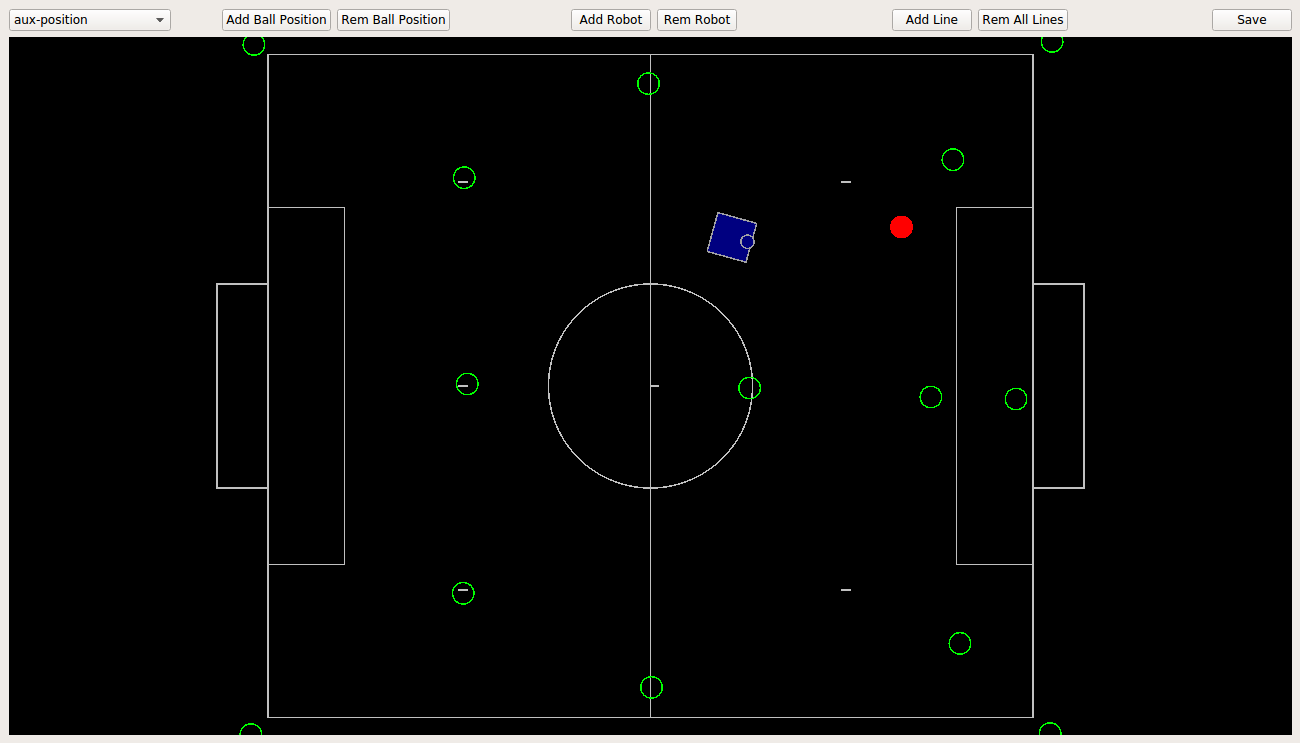
\includegraphics[width=1.05\textwidth]{figures/delaunay_interface.png}
   \caption{Interface para posicionamento com triangulação de Delaunay.} \label{fig:delaunay_interface}
\end{figure}

\item Os valores dessas posições são guardadas em um arquivos de texto para posterior uso no código da estratégia. Um exemplo desse arquivo de configuração se encontrar na figura \ref{fig:text_config_delaunay}, em que temos 2 jogadores em três posições, como escrito na linha 1 do arquivo; seguido pela localização da bola, com apenas as coordenadas x e y, e as posições dos jogadores, com as coordenadas x,y e ângulo. Essas localizações são repetidas três vezes conforme escolhido (linha 1).

\begin{figure}[H]
	\centering
	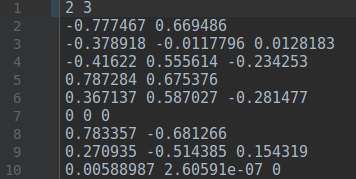
\includegraphics[width=0.8\textwidth]{figures/text_config_delaunay.png}
   \caption{Arquivo de configuração para posicionamento dcom triangulação de Delaunay.} \label{fig:text_config_delaunay}
\end{figure}

\item A estratégia do auxiliar utiliza a triangulação de Delaunay para a posição atual da bola, em conjunto com o arquivo de configuração feito, para interpolar as posições discretas escolhidas e fazer que o algoritmo retorna uma posição ótima independente da localização da bola.

\item Com a posição obtida pela triangulação, é usado o algoritmo de planejamento de trajetórias RRT, em conjunto com o seu controlador, para chegar nessa posição interpolada.

\end{enumerate}

\subsection{Táticas de Jogo}

Táticas de Jogo, representado pela classe 'Play', é a parte mais alto nível da estratégia. Essa classe é responsável por escolher qual técnico usar em um determinado momento da partida. O Play escolhe qual o melhor modo de se jogar em uma situação, como, por exemplo, ter uma postura mais agressiva ou mais defensiva envolvendo os três jogadores. Só pode existir um Play no jogo, que pode ser tratado como a raiz de uma Behavior Tree que tem os técnicos como filhos, tendo, cada um, três árvores relativas a cada jogador.

O seu funcionamento é similar ao Selector Behavior, no sentido em que é preciso escolher apenas um técnico a cada momento. Para avaliar quando é necessário fazer uma troca, usa-se o mesmo modelo de retorno: TRUE, FALSE e RUNNING para os técnicos. 

Dado essa troca, pode ser criados técnicos temporários para jogadas específicas de jogo, como o goleiro sair do gol e voltar outro jogador, que é uma ação de transição. Isso pode significar que um técnico principal pode chamar esse outro, voltando depois para o mesmo técnico novamente. Então, podemos ter um técnico principal e vários temporários para jogadas ensaidas e específicas que envolvam mais de um jogador.


\section{Resultados Obtidos}
	\label{secao: resultados_obtidos}
    
Nessa seção, são apresentados os resultados obtidos na resolução do problema da tomada de decisão para robôs jogadores de futebol IEEE Very Small Size Soccer. Os resultados a seguir foram obtidos estudando o comportamentos de equipes adversárias na competição, além de diversos testes com o time de robôs da ITAndroids contra si mesmo em simulações computacionais em um simulador feito pela própria equipe, como mostrado na figura \ref{fig:simulator}.

\begin{figure}[H]
	\centering
	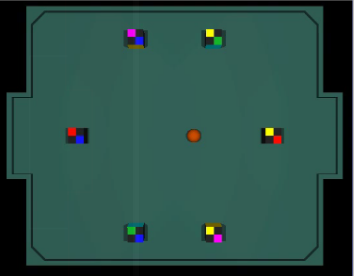
\includegraphics[width=0.6\textwidth]{figures/SimulatorWithoutButtons.png}
	\caption{Simulador da ITAndroids.}
	\label{fig:simulator}
\end{figure}

\subsection{Papéis}

Aqui, será apresentado os papéis criados para a competição e as árvores de comportamento criadas para cada um deles.

\subsubsection{Goleiro}

A BT criada para o goleiro está representada na figura \ref{fig:goalier_bt}.

\begin{figure}[H]
	\centering
	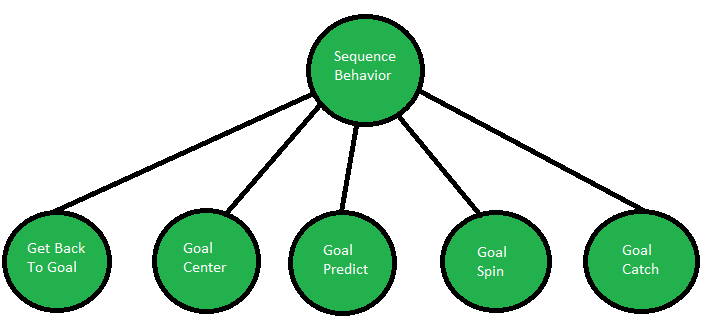
\includegraphics[width=0.8\textwidth]{figures/Goalier_BT.png}
   	\caption{Behavior Tree para o goleiro.} \label{fig:goalier_bt}
\end{figure}

Como visto, ela é composta por um nó do tipo Sequence Behavior, que irá executar os seus filhos em sequência. Esse papel, então, executa as seguintes ações prioritando as primeiras a aparecerem na seguinte lista:

\begin{itemize}

\item \textbf{Get Back to Goal Behavior} Volta para o gol, caso que, se por algum motivo ele esteja fora do próprio.

\item \textbf{Goal Center} Fica centralizado no gol quando a bola estiver longe, de forma que o jogador possa rapidamente ir para qualquer um dos lados quando a bola se aproximar.

\item \textbf{Goal Predict} Prediz para onde a bola irá quando ela estiver rápida e longe do gol.

\item \textbf{Goal Spin} Gira quando está perto da bola e não tem oponente perto da bola para jogá-la para longe.

\item \textbf{Goal Catch} Comportamento que o goleiro deverá fazer quando não fizer nenhum outro, por isso sua última posição na sequência. Ele acompanha o movimento da bola com o goleiro sobre a linha do gol.

\end{itemize}



\subsubsection{Principal}

Já para o principal, a árvore \ref{fig:principal_bt} foi desenvolvida, sendo a árvore mais complexa dentre os papéis.

\begin{figure}[H]
	\centering
	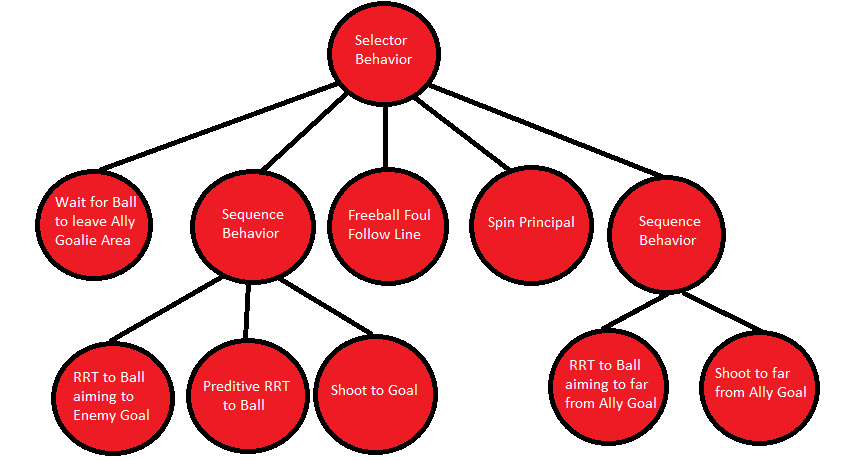
\includegraphics[width=0.8\textwidth]{figures/Principal_BT.png}
   	\caption{Behavior Tree para o principal.} \label{fig:principal_bt}
\end{figure}   

Conforma a figura \ref{fig:principal_bt}, a raiz da árvore do principal é um Selector Behavior que escolhe uma das ações a ser realizada. Essa BT tem mais dois outros nós compostos, que são dois Sequence Behavior usados para o posicionamento atrás da bola, seguido pelo chute. Uma descrição dos nós folha utilizados se encontra abaixo:

\begin{itemize}

\item \textbf{Wait for Ball to leave Ally Goalie Area} Esse Behavior utiliza a Triangução de Delaunay, com a mesma interface desenvolvida na figura \ref{fig:delaunay_interface}. Esse comportamento deve evitar que o jogador entre na área do goleiro para não sofre penalty, conforme descrito na figura \ref{fig:penalty}. O jogador se pocionará de acordo com posições escolhidas pelo usuário, calibradas com o arquivo de configuração do mesmo modelo da figura \ref{fig:text_config_delaunay}.

\item \textbf{RRT to Ball aiming to Enemy Goal} Irá usar o algoritmo de planejamento de trajetórias RRT para se deslocar atrás da bola com direção apontando para o gol oponente. Usado para se aproximar da bola e, em seguida, trocar para o próximo behavior, o Predictive RRT to Ball.

\item \textbf{Predictive RRT to Ball} Usa uma predição linear considerando que a bola continuará na mesma velocidade. Usado para se chegar na bola com mais precisão quando próximo a ela. Chega atrás da bola mirando para o gol.

\item \textbf{Shoot to Goal} Esse behavior só é chamado quando o jogador já está alinhado com a bola e o gol oponente. Esse comportamento acelera rapidamente o robô em linha reta para chegar no gol com uma velocidade alta.

\item \textbf{Free Ball Foul Follow Line} Esse behavior é um específico para situações de falta do tipo Bola Livre, conforme descrito em \ref{fig:bola_livre}. Quando for detectado uma dessas posições, o jogador deve acelerar o mais rápio possível em direção à bola para ter o controle dela antes do oponente.

\item \textbf{Spin Principal} Esse nó deve ser chamado quando a bola estiver em um dos quatros campos do campo. Caso seja um campo defensivo, o jogador irá girar para jogar a bola para frente; caso seja um na zona de ataque, o jogador girará para por a bola no centro do campo e continuar o ataque.

\item \textbf{RRT to Ball aiming to far from Ally Goal} Irá usar o algoritmo de planejamento de trajetórias RRT para se deslocar atrás da bola com direção apontando para a zona de ataque (longe do gol aliado). Usado para se aproximar da bola e se posicionar para, em seguida, chamar o Behavior Shoot to Far from Ally Goal.

\item \textbf{Shoot to Far from Ally Goal} Esse behavior só é chamado quando o jogador já está alinhado com a bola e o para frente (para longe do gol alidado). Esse comportamento acelera rapidamente o robô em linha reta para por a bola na zona de ataque.

\end{itemize}


\subsubsection{Auxiliar}

O auxiliar, por sua vez, tem uma Behavior Tree muito simples, representada por apenas um nó que tem como função se posicionar em lugar ótimo com Triangulação de Delaunay\cite{delaunay34}. Sua árvore, é representada simplesmente pela figura \ref{fig:auxiliar_bt}.

\begin{figure}[H]
	\centering
	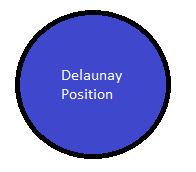
\includegraphics[width=0.4\textwidth]{figures/Auxiliar_BT.png}
   \caption{Behavior Tree para o auxiliar.} \label{fig:auxiliar_bt}
\end{figure}


\subsection{Técnicos}

Finalmente, será mostrado quais técnicos foram usados na estratégia. A princípio, três técnicos foram desenvolvidos. Primeiramente, será descrito o comportamento de cada um deles e quando é esperado que cada um seja usado, seguido das condições de troca entre eles.



\subsubsection{Dois principais} Esse técnicos usa uma formação de jogadores com 1 goleiro e dois jogadores principais. Isso significa que os dois principais irão para à bola ao mesmo tempo, o que pode ser caótico para uma situação de ataque, em que precisão para acertar a bola é necessária. Porém, para situaçõe defensivas, esse técnico demonstra muita eficácia, porque os dois jogadores se tornam efetivamente zagueiros, indo para a bola e dificultando o avanço do atacante adversário.

\subsubsection{Um principal e um auxiliar} Esse técnico, diferente do anterior, é usado para situações de ataque. Ao utilizar apenas um principal, essa formação é capaz de fornecer ataques muito mais precisos, em que os jogadores aliados não se colidem durante a movimentação. O auxiliar, nessa formação, não fica muito longe da bola, ficando esperando a bola escapar do principal, por uma defesa do oponente por exemplo. No momento que o auxiliar estiver em uma posição mais próxima da bola que o principal, ele se torna o principal, enquanto que o principal se torna o auxiliar, de modo que o ataque seja contínuo. Essa formação se mostrou muito eficaz na CBR, fazendo que a ITAndroids tivesse um dos ataques, em termos de estratégia, mais consistentes da competição.

\subsubsection{Troca de Goleiro} Esse é um tipo de técnico temporário para realizar uma jogada específica de jogo, sendo feito para uma ação de transição. Esse técnico será chamado em situações em que o goleiro deverá sair do gol e se tornar um principal, enquanto que o outro jogador mais próximos do gol se torna o novo goleiro. A situação em que essa troca deve ocorrer é quando a bola está perto do goleiro e todos os jogadores inimigos estão bem longe, condição necessária por se tratar de uma jogada arriscada.

Tecnicamente, esse técnico é usado em situações em que temos 2 principais e um goleiro, já que ele só ocorrer em situações defensivas. Ele funciona fazendo que o goleiro se torne o principal sem o Behavior de esperar a bola sair do gol, como mostrado na figura \ref{fig:OutOfGoal_BT}. Em seguida, o jogador principal mais próximo do gol se torna um goleiro e, como ele está fora do gol, voltará para tal por meio do Behavior Get Back to Goal. Quando o novo goleiro chegar em sua posição, esse técnico é terminado e volta para o técnico que estava anteriormente.

\begin{figure}[H]
	\centering
	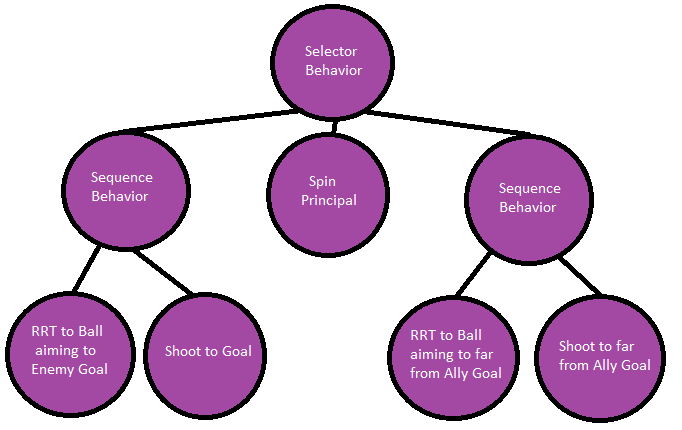
\includegraphics[width=0.8\textwidth]{figures/LastGoalierOutOfGoal.png}
   	\caption{Behavior Tree usada para o goleiro quando este sai do gol.} \label{fig:OutOfGoal_BT}
\end{figure}


\section{Conclusões}

O projeto de Iniciação Científica apresentou bons resultados, especialmente quanto à vitória da equipe do ITA até às quartas de final da CBR 2017, rendendo o sétimo lugar à equipe dentre mais de 25 equipes participantes. Além do fato de que a ITAndroids conquistou o primeiro lugar na competição nacional de VSSS Copa Turing 2017, que ocorreu no final de setembro de 2017.

Do ponto de vista técnico, o uso do algoritmo da Behavior Tree, já consagrado e usado por times de nível mundial, se mostrou factível e funcional em partidas reais de competições. Contudo, problemas como pouca escalabilidade e pouca reutilizabilidade se mostraram presentes na estratégia desenvolvida. Isso significa que mudanças ainda deverão ser feitas nas BT, principalmente a respeito do uso de mais nós do tipo paralelo para remover esses problemas citados.

\section{Agradecimentos}

\begin{itemize}
\item Ao CNPq, pelo apoio financeiro e motivacional.
\item À ITAndroids, equipe que representa o ITA na competição da LARC/CBR, pela ideia do projeto, pela disponibilidade do robô real para implementação e oportunidade de aplicação dos métodos estudados.
\item Ao professor doutor Paulo Marcelo Tasinaffo, meu orientador, e ao professor doutor Marcos Ricardo de Omena Máximo, co-orientador, ambos da Divisão da Ciência da Computação do ITA, pelo apoio nos estudos e no desenvolvimento do projeto.

\end{itemize}

\section{Bibliografia}

\printbibliography


\end{document}